\documentclass{article}
\usepackage[nonatbib, preprint]{neurips}
\usepackage[T1]{fontenc}        % use 8-bit T1 fonts
\usepackage[utf8]{inputenc}     % allow utf-8 input

\usepackage{booktabs}           % professional-quality tables
\usepackage{enumerate}          % lists
\usepackage{microtype}          % microtypography
\usepackage{todonotes}          % todos
\usepackage{url}                % simple URL typesetting

% Math
\usepackage{amsmath}            % misc math
\usepackage{amssymb}            % blackboard math symbols
\usepackage{amsthm}             % theorems
\usepackage{mathtools}          % enhance the appearance of math
\usepackage{xfrac}              % compact symbols for 1/2, etc.
\DeclareMathOperator*{\argmin}{argmin}
\DeclareMathOperator*{\argmax}{argmax}
\allowdisplaybreaks

% Graphics, Plots
\usepackage{graphicx}           % graphics
\usepackage{subcaption}         % subcaptions
\usepackage{epsfig, epstopdf}   % subfigures

% Colors
\usepackage{xcolor}

% Hyperlinks and bookmarks
\usepackage{hyperref}
\usepackage[capitalize]{cleveref}
\hypersetup{
  bookmarksopen={true},
  colorlinks={true},
  linkcolor={blue!80!black},
  citecolor={green!50!black},
  urlcolor={blue!80!black}
}

% Setup title
\title{Exploring evolutionary protein fitness landscapes}
\author{
  Ayush Karnawat \\
  Department of Electrical Engineering and Computer Science \\
  Case Western Reserve University,
  Cleveland, OH 44106 \\
  \texttt{axk840@case.edu} \\
}

\begin{document}
\maketitle

% Abstract
\begin{abstract}
  The ability to efficiently design protein for a specific purpose -- namely for
  therapeutic and other industrial applications -- has long been the dream of
  chemical and bioengineers. Conventional experimental techniques such as
  directed evolution, while highly percise, are unable to find rare, enhanced
  variants of the protein of interest. Here, we investigate how a
  semi-supervised adaptive sampling approach can be used to effectively explore
  the search space, in order to improve protein design. Unlike other black-box
  predictive models, which are known to suffer from bias introduced in the
  training distribution, our model does not directly optimize the oracle to
  improve its predictive power. Rather, it estimates a distribution over the
  design space conditioned on the desired properties. Using the streptococcal
  protein G's $\beta 1$ (GB1) domain as an illustrative example, we demonstrate
  how machine-guided protein design can efficiently navigate the landscape to
  locate non-trivial high-fitness protein designs. Overall, our approach is a
  first step toward enabling efficient use of expensive laboratory experiments
  without sacrificing throughput.
\end{abstract}
% \keywords{Bayesian Inference \and Adaptive Sampling \and Protein Engineering
%           \and Fitness Landscape}


% Introduction
\section{Introduction}
Proteins are the inherent building blocks of all life, and play a highly
critical role as molecular machines in cells by sensing, signaling, and
catalyzing chemical reactions. Due to their extensive design capabilities
\cite{dahiyat1997novo, jackel2008protein} -- such as to maximize binding
affinity to a target -- they have been subject to a lot of trail and error
experimentation, which is not only a time-consuming, but also costly procedure.
In fact, according to \cite{dimasi2016innovation}, it takes an average of 12
years and $\sim\$2.6$ billion USD to design a effective drug, with costs rising
each year \cite{dickson2009cost}. 

Recent advances in computational protein design have showed great promise in
this regard by creating novel proteins \textit{de novo} \cite{huang2016coming}.
However, a closer inspection reveals its design range is (currently) limited to
simple folds and static structures, which is only a small subset of proteins in
the vast design space \cite{pierce2002protein}. As such, improving design
through directed evolution, a technique introduced in \cite{chen1991enzyme} and
further popularized by \cite{romero2009exploring}, is still used today. Here, in
a iterative manner, random mutations (chosen uniformly from the search space)
from a parent population of proteins are induced, properties of interest are
measured, and the top $k$ variants are chosen for the next round of mutations.
While this approach has high-fidelity, it is (a) dependent on resource intensive
assays, and (b) unlikely to be efficient in finding the best design from the
search space.

One way to improve this is to apply computational methods to certain aspects of
the design cycle \cite{gomez2018automatic, schneider1998peptide, biswas2020low,
yang2018machine, alley2019unified}. For example, a trivial place to employ a
purely computational approach is to replace the laboratory assays with an
``oracle'' that can accurately predict the property of interest. However, this
relies on the regression oracle being well-behaved, even in regions of the
search space far from the initial training dataset. Yet, recent work has shown
how brittle state-of-the-art (SOTA) image \cite{moosavi2016deepfool,
nguyen2015deep} and text \cite{liang2017deep, behjati2019universal}
classification models can be due to pathological biases introduced by the
training distribution, especially for inputs not in the original training set
\cite{amini2019uncovering, cisse2017houdini}. As such, approaches that directly
optimize the predictive oracle can be led astray into regions of the search
space that are poor, resulting in unreliable sequences, i.e. proteins that are
intrinsically unfolded or unable to fold properly. To avoid this issue, one can
use an optimization scheme that incorporates prior information using a bayesian
approach \cite{gunawan2006bayesian, mockus2012bayesian}. This can be seen as an
way to encode knowledge about either (a) the regions where the oracle is
expected to be accurate (i.e. by learning the distribution of the training
dataset), or (b) what constitutes a ``realistic'' input (i.e. by learning
representations of proteins known to stably fold).

A (potentially) more well-suited modification to the directed evolution method,
which involves optimizing how the search space is traversed, is likely to find
better designs. Although directed evolution is adept at searching and climbing
nearby peaks within a local neighborhood \cite{romero2009exploring}, it is not
conducive to finding functional neighborhoods far away from the original parent
sequence \cite{pokusaeva2017experimental}, due to the fact that many randomly
sampled sequences are non-functional \cite{keefe2001functional, du2016good}.
This is further exacerbated by the fact that, as the length $L$ of the protein
increases, the design space becomes exponentially vast (scaling $\Theta
(20^L)$), making an exhaustive random search intractable. There is, hence, an
opportunity to use a combinatorial optimization technique to explore the design
space more efficiently \cite{baluja1997using, schneider1997search}, while also
taking into account the exploration-exploitation (EvE) tradeoff
\cite{chen2009optimal, sabharwal2012guiding}.

A class of methods, based on variants of the Monte Carlo (MC) approach, that
account for the EvE tradeoff have been used extensively to explore large search
spaces (e.g. Scrabble words \cite{sheppard2002world} or Go moves
\cite{gelly2012grand, silver2017mastering}) to a high degree of effectiveness.
However, performing the tree search requires that the evalutation be
deterministic for a specific state of the positions \cite{gelly2006exploration}.
Contrarily, in our design task, -- and more generally for most real-world design
problems -- the evaluation function is typically a stochastic approximation of
the ground truth. Therefore, we require that the uncertainty be leveraged within
our method to achieve proper optimization \cite{brookes2018design}. 

One way to ensure this is to formulate the approach using evolution strategy
(ES) algorithms \cite{back1996evolutionary}, which are known to handle a wide
range of uncertainties \cite{jin2005evolutionary}, such as changes to the
environment (i.e. design space) or noisy ``oracle'' function evaluations. In
particular, the Covariance Matrix Adaptation Evolution Strategy (CMA-ES)
\cite{hansen1996adapting} allows for black-box optimization of non-linear
non-convex functions, such as a protein's rugged evolutionary landscape
\cite{macken1989protein}. Here, new candidate sets are sampled according to a
multivariate gaussian distribution in $\mathbb{R}^{n}$. After the points are
evaluated, the mean ($\mu$) and the variance ($\sigma^2$) of the mutivariate
gaussian are updated to provide (potentially better) samples for the next
iteration. This is repeated until either (1) no feasible set of samples is found
or (2) a tolerance criteria is met between the changing $\mu, \sigma^2$. Akin to
CMA-ES, we instead use a SOTA optimization algorithm based on
\cite{brookes2018design}, which extends beyond the multivariate gaussian to a
more general set of underlying generative models. This allows us to use, for
example, Variational Autoencoders (VAEs) \cite{kingma2013auto} or Generative
Adverserial Networks (GANs) \cite{goodfellow2014generative} to more effectively
generate plausible sequences from the search space.
% TODO: Should we write a more mathematically detailed approach to how variants
% are sampled using the CMA-ES approach.
% Talk about how the CMA sampling draws froma gaussian distributon, whereas we
% want to generalize it to a learned conditional distribution, so that we can more
% effectively generate the "right" samples.

As alluded to previously, the biggest benefit this approach brings over a
conventional optimization technique is that it saves resources (in both time and
money) since we don't waste time querying\footnote{We do not want to keep
exploring the search space if there is no benefit from doing so.} poor regions
of the search space \cite{sareni2000efficient}. Additionally, since the fitness
evaluation function is derivative-free, i.e. a black box that provides a simple
input to ouput mapping, a wet-lab protein assay can easily be used inplace of
the oracle\footnote{Careful consideration should be placed on the inherent
variance induced by different assay types \cite{noble2009quantitation}. In fact,
by design, the optimization procedure uses this variability to address the
concern that the oracle is a stochastic approximation of the ``true'' fitness
value. For further detail see $\S$\ref{sec:methods}.}, to more accuratey
optimize the design. This allows our method to be scalable in a real-world
protein design context.

Overall, in this work, we explore the benefits and drawbacks of using an
adaptive sampling technique based on a bayesian inference framework to navigate
the protein's fitness landscape. We think this approach, owning to the use of a
SOTA optimization technique, can considerable accelerate the evolutionary design
process, thus reducing resource intensive tasks, such as assay preparation and
quantification. We demonstrate our ideas empirically using protein variants of
the $\beta 1$ domain of the G protein as a test case \cite{wu2016adaptation}.
Here, the fitness is a proxy for the stability (i.e. the fraction of folded
proteins) and function (i.e. binding affinity to IgG-Fc) of the domain. We hope
to inspire a hybrid approach where the adaptive sampling portion of the
optimization strategy is used in conjunction with actual wetlab results to gain
an accurate picture of the protein fitness landscape.


\section{Methods}
\label{sec:methods}

\subsection{Problem definition}
\label{sec:methods-problem_definition}
We consider the problem of finding instances of an $L$-dimensional random vector
(i.e. a protein sequence) that satisfies a certain design criteria. The criteria
is highly problem dependent; most commonly, we are concerned with the
maximization (i.e. finding a protein that is maximally fit) or the specification
property (i.e. designing a protein that has a certain binding affinity). In our
formulation, since proteins are just sequences defined by a vocab, we assume
that our dataset $X$ is discrete with samples $x \in \mathbb{N}^L$. However, as
will be evident from the mathematical description, we can also work with the
structural representation of proteins (represented as $n$-order tensors) with
realizations $x \in \mathbb{R}^{I_1 \times \dots \times I_n}$.

To build our predictive models, we assume access to realizations $x \in X$ drawn
from an unknown underlying data distribution, $p_D(x)$, denoted as the training
set. Our hope is that this will help us build a certain class of generative
models, $p(x|\theta)$, that can approximate $p_D(x)$ well\footnote{Here,
``well'' is a particulary fuzzy term; by it we mean that the samples generated
are similar to the training set. A more mathematically accurate definition can
be found in $\S$\ref{sec:methods-generative_model_optimization}.}. We define the
parameters of this model by $\theta^{(0)}$ after it has been fit to the data,
which yields our prior density $p(x|\theta^{(0)})$.

In addition to a generative model, we assume that, to properly optimize how the
search space is travered, we are given a predictor $p(y|x)$ (hereby named an
``oracle''). This provides a distribution over the property of interest $y$
given a particular realization $x \in X$. From this oracle, we should be able to
calculate the probability of events contained in $S$ occuring. Note that $S$
changes depending on the problem criteria. In particular, for maximization
problems, $S$ contains the set of values $y$ such that $y \geq y_{max} \equiv
\max_{x} \mathbb{E}_{p(y|x)}[y]$. Less stringently, following
\cite{brookes2019conditioning}, we consider the set $S = \{y | y \geq y^* \leq
y_{max} \}$, where $y^*$ is some predefined threshold or taken to be the
quantile of the data. Regardless of the how the design criteria is specified,
our ultimate aim is to condition the prior density on our desired property
values $p(S|x,\theta^{(0)})$ and sample from the resulting distribution. This
will ensure that the generated samples are realistic samples (i.e. variants
found in nature) assuming that the resulting conditional can be
well-approximated using an accurate generative model $q(x|\phi)$. As the
optimizaton procedure evolves, the parameters $\phi$ will move towards values
that approximate the desired conditional density well.


\subsection{Generative model optimization}
\label{sec:methods-generative_model_optimization}
Since we are interested in the maximization property for our experiments, we
focus here on maximizing our expected probability, $P(S|\theta)$, over the
property values. Note that a similar formulation can be derived to optimize the
probabilty for the specification problem. More specifically, we solve the
following optimization problem,
%
\begin{align}
  \hat{\theta}
    &= \argmax_{\theta} \log P(S|\theta) \\
    &= \argmax_{\theta} \log \int p(S|x) p(x|\theta) dx \\
    &= \argmax_{\theta} \log \mathbb{E}_{p(x|\theta)} [P(S|x)] \label{eq:basic_opt}
\end{align}
%
which, if all the underlying inputs are well-behaved, would allow us to easily
find our ``desired'' input $\hat{x}$ from the posterior distribution, i.e.
$\hat{x} \sim p(x|\hat{\theta})$. However, the biggest problem with this
approach lies in the fact that our desired property $S$, by nature, is a rare
condition, thereby making the probability $P(S|\theta)$ extremely small for most
parameters $\theta$ of the generative model. This makes it hard to optimize and
can result in high-variance predictions from the ``oracle'', especially when
there are not enough samples in the training set.

To remedy this, we begin by iteratively optimizing (\ref{eq:basic_opt}) using
$\theta^{(t)}$, where, at each iteration $t$, the generative model
$p(x|\theta^{(t)})$ becomes closer and closer to the desired conditional
distribution. In fact, to estimate our conditional, we make use of our prior
model conditioned onto the set of values $S$ using Bayes' theorem,
%
\begin{equation}
  p(x|S, \theta^{(0)}) = \frac{P(S|x) p(x|\theta^{(0)})}{P(S|\theta^{(0)})} 
  \label{eq:bayes}
\end{equation}
%
where $P(S|\theta^{(0)}) = \int P(S|x) p(x|\theta^{(0)}) dx$. Then, to find the
ideal set of parameters $\phi^*$ for the generative model (which acts as the
``search'' model), we minimize the KL divergence between the target conditional
$p(x|S,\theta^{(0)})$ and the search model, $q(x|\phi)$,
%
\begin{align}
  \phi^*  &= \argmin_{\phi} D_{KL} \Big[ p(x|S,\theta^{(0)}) || q(x|\phi) \Big]
              \label{eq:kld_optim} \\
          &= \argmin_{\phi} \int p(x|S,\theta^{(0)}) \log 
              \left[ \frac{p(x|S,\theta^{(0)})}{q(x|\phi)} \right] dx \\
          &= \argmin_{\phi} \underbrace{\int p(x|S,\theta^{(0)})
              \log[p(x|S,\theta^{(0)})] dx}_{H_0}
              - \int p(x|S,\theta^{(0)}) \log[q(x|\phi)] dx \\
          &= \argmax_{\phi} \int p(x|S,\theta^{(0)}) \log[q(x|\phi)] dx \\
          &= \argmax_{\phi} \int \frac{P(S|x) p(x|\theta^{(0)})}
              {P(S|\theta^{(0)})} \log[q(x|\phi)] dx \\
          &= \argmax_{\phi} \frac{1}{P(S|\theta^{(0)})} \int p(S|x) 
              p(x|\theta^{(0)}) \log[q(x|\phi)] dx \\
          &= \argmax_{\phi} \mathbb{E}_{p(x|\theta^{(0)})} [p(S|x) 
              \log q(x|\phi)] \label{eq:interim_opt}
\end{align}
%
Note that $P(S|\theta^{(0)})$ and $H_0$ are removed from the overall objective
since they do not rely on the optimization parameter $\phi$. In most cases,
(\ref{eq:interim_opt}) is the function we want to optimize, but, as mentioned
previously, it doesn't take into account if $S$ is a rare property. To address
this, we use an importance sampling distribution, where rare samples are given
higher probability versus more common samples, and rewrite our objective
function as,
%
\begin{align}
  &\argmax_{\phi} \mathbb{E}_{r(x)} \left[ \frac{p(x|\theta^{(0)})}{r(x)}
    p(S|x) \log q(x|\phi) \right] \\
  &\argmax_{\phi} \mathbb{E}_{r^{(t)}(x)} \left[ \frac{p(x|\theta^{(0)})}{
    r^{(t)}(x)} p(S^{(t)}|x) \log q(x|\phi) \right] \label{eq:iter_opt}
\end{align}
%
by adding an iteration dependence $t$ on both $S^{(t)}$ and $r^{(t)}(x)$. This
ensures that $\mathbb{E}_{r^{(t)}(x)} [P(S^{(t)}|x)]$ has non-vanishing
probability, meaning that we can draw samples $x \sim r^{(t)}(x)$ that have
reasonably high values of $P(S^{(t)}|x)$. Additionally, this allows for
$S^{(t)}$ to approach $S$ as $t$ grows large ($S^{(t)} \supset S^{(t+1)} \supset
\dots \supset S$). 

For the first iteration ($t=0$) of the algorithm, we set (a) $S^{(0)}$ to be the
property values that are greater than the $Q^{\text{th}}$ percentile of the
oracle values predicted for the training sample, i.e. $S^{(0)} = p(y \geq
\gamma^{(0)} | x)$ and (b) the importance sampling distribution to the prior,
i.e. $r^{(0)}(x) = p(x|\theta^{(0)})$. This helps us build the approximate
conditional $q(x|\phi^{(0)})$. Similarly, for the remaining iterations, we set
(a) $\gamma^{(t)}$ to the $Q^{\text{th}}$ percentile of the property values of
the samples $x^{(t)}$ generated from the previous iterations search distribution
$q(x|\phi^{(t-1)})$, and (b) $r^{(t)} = q(x|\phi^{(t-1)})$. Substituting these
in, (\ref{eq:iter_opt}) becomes
%
\begin{equation}
  \phi^{(t+1)} = \argmax_{\phi} \mathbb{E}_{q(x|\phi^{(t)})} \left[
    \frac{p(x|\theta^{(0)})}{q(x|\phi^{(t)})} P(S^{(t)}|x) \log q(x|\phi)
  \right] \label{eq:final_exact_opt}
\end{equation}
%
which can be approximated by drawing $M$ random samples from the search model,
$x_{i}^{(t)} \sim q(x|\phi^{(t)})$ for $i = 1, \dots, M$,
%
\begin{equation}
  \phi^{(t+1)} = \argmax_{\phi} \sum_{i=1}^{M} \frac{p(x_{i}^{(t)}|\theta^{(0)})}{
    q(x_{i}^{(t)}|\phi^{(t)})} P(S^{(t)} | x_{i}^{(t)}) \log q(x_{i}^{(t)} | \phi)
  \label{eq:final_approx_opt}
\end{equation}
%
It is necessary in this approximation that the property values $P(S^{(t)}|x)$ be
non-zero and the ratio $\frac{p(x | \theta^{(0)})}{q(x | \phi^{(t)})}$
well-behaved. Luckily, this is satisfied by the weighting scheme itself, which
ensures that the density of the search model, $q(x|\phi)$, is close to the prior
distribution, $p(x|\theta^{(0)})$, through minimization of the KL divergence as
shown in (\ref{eq:kld_optim}). 


\subsection{Connection to latent variable models}
\label{sec:methods-latent_variable_models}
The objective presented in (\ref{eq:final_approx_opt}) requires us to accurately
calculate the density of the prior, $p(x|\theta^{(0)})$, and the search model,
$q(x|\phi)$, for any input $x$. For certain classes of latent variable models
this is not possible, since marginalization over the latent space is
intractable. However, if both the densities are defined on the same latent
space, $z$, then one can evaluate the joint densities of the observed and latent
variables by computing $p(x,z|\theta^{(0)})$ and $q(x,z|\phi^{(t)})$. This is
possible due to the well-known fact that an expectation over the marginal is
equal to the expectation over the joint, i.e. $\mathbb{E}_{p(x)}[f(x)] =
\mathbb{E}_{p(x,y)}[f(x)]$. Using this result, we can reformulate our objective
as,
%
\begin{align}
  \phi^{(t+1)}  &= \argmax_{\phi} \mathbb{E}_{q(x,z|\phi^{(t)})} \left[
                    \frac{p(x,z|\theta^{(0)})}{q(x,z|\phi^{(t)})} P(S^{(t)}|x)
                    \log q(x|\phi) \right] \label{eq:latent_exact_opt} \\
                &= \argmax_{\phi} \sum_{i=1}^{M} \frac{p(x_{i}^{(t)},z_{i}^{(t)}
                    |\theta^{(0)})}{q(x_{i}^{(t)}, z_{i}^{(t)}|\phi^{(t)})} 
                    P(S^{(t)} | x_{i}^{(t)}) \log q(x_{i}^{(t)} | \phi)
                    \label{eq:latent_approx_opt}
\end{align}
%
which is optimized in a similar fashion to (\ref{eq:final_approx_opt}); the only
difference being that $x_{i}^{(t)}, z_{i}^{(t)} \sim q(x,z|\phi^{(t)})$.


\subsection{Performance measures}
\label{sec:methods-performance_measures}
To measure how well our overall objective traverses the search space, we first
compute the fitness $w$ for a given variant $x$ as,
%
\begin{equation}
  w(x) = \frac{\frac{\text{count}_{x,\text{selected}}}{\text{count}_{x,\text{input}}}}
    {\frac{\text{count}_{\text{WT, selected}}}{\text{count}_{\text{WT, input}}}}
  \label{eq:fitness}
\end{equation}
%
where $\text{count}_{x,\text{selected}}$ and $\text{count}_{x,\text{input}}$
represent the count of variant $x$ in the selected library and input library,
respectively. Similarly, $\text{count}_{\text{WT, selected}}$ and
$\text{count}_{\text{WT, input}}$ represent the count of the WT in the selected
and input libraries. Here, the fitness of each variant is normalized relative
the WT sequence fitness score. Note that, since the regression-based oracle
gives us a equivalent calculation via a mapping $f: \mathbb{R}^L \to
\mathbb{R}$, we do not actually compute the fitness score using
(\ref{eq:fitness}).

We want to use this score to visualize the fitness landscape for different
inputs $x$. However, with a one-dimensional visualization, it is hard to
understand which collection of variants are more ``fit'' than others. Naively,
one could view the sequences in 2D space, where each sequence (inserted
iteratively) represents a entry in 2D space. But this representaton is poor at
preserving groups; instead, we want a projection that maintains the locality of
the data points (i.e. sequences close to each other in 1D space should remain
close to each other in the 2D representation). As it turns out, using a Hilbert
curve \cite{hilbert1935stetige}, with order $\eta$ determined by the total
number of datapoints $n$,\footnote{We kindly refer to $\S 2.4$ in
\cite{sagan2012space} for a detailed derivation of how the 2D coordinates for
the curve are generated.}
%
\begin{equation}
  \eta = \left\lceil \frac{\log \sqrt{n}}{\log 2} \right\rceil
  \label{eq:hilbert_order}
\end{equation}
%
allows for a locality-preserving mapping $\varphi: \mathbb{R}^1 \to
\mathbb{R}^2$ \cite{moon2001analysis}. Through this projection, we are able to
spatio-temporally understand which collection of sequences are being queried by
the search model $q(x|\phi^{(t)})$ for each iteration $t$.


\section{Experiments}
\label{sec:experiments}
To demostrate the benefits of this approach, we focus on the problem of
maximixation of a protein's fitness, although, as mentioned above, specification
of a particular frequency can also be optimized. We systematically compare our
approach to the widely-used random sampling technique found in directed
evolution on a set of protein variants taken from the $\beta 1$ domain of the G
protein \cite{wu2016adaptation}.

In order to compare the methods, it was necessary to evaluate the data with a
known ground truth since evaluating on a held-out test set was not feasible for
our problem. To obtain a (somewhat) accurate ground truth model, we trained a GP
regressor (GPR) on the same training data as the oracle using a kernel designed
for protein-related tasks \cite{shen2014introduction}, whose features space was
augmented by adding a bias feature and exponentiating to obtain a second-order
kernel. We make this modification because a protein's fitness scores (for its
variants) typically follow a nonlinear function \cite{hu2004developing}. The
ground truth fitness score was taken to be the mean of this GPR model and logged
for comparison. 

To optimize our method properly, we selected an oracle, GPR combination pair
that was trained on the same subset of data. We stress, here, that we do not use
different subsets of the the data for each model because we want to ensure that
we do not cherry-pick the parameters of our predictive models. For the VAE
model, however, we used the full dataset because it was trained in an
unsupervised fashion only for the context of generating new sequences that are
similar to original dataset. \cref{tab:random_vs_designed_topk} shows the top 10
sequences (based off the oracle values), obtained by both the directed evolution
(randomly-sampled) and the CbAS (adaptive sampling) method. While both methods
reached approximately similar oracle and GT value scores, the latter reached the
``optimal'' variants more efficienty, requiring less oracle queries, as evidence
by the more localized search in \cref{fig:landscape_hilbert}. This, as mentioned
previously, will be especially useful in a real-world setting where querying
resource-intensive assays to assess a variant's fitness might be unfeasible for
most proteins. 

\begin{table}[htbp]
  \centering
  \resizebox{\textwidth}{!}{%
  \begin{tabular}{@{}cccccccccccc@{}}
  \toprule
  Method & \multicolumn{1}{l}{} & \multicolumn{10}{c}{Top $k$ fitness scores (oracle)}                                    \\ \midrule
         & Sequence             & QWAA   & SWRA   & QWGM   & IWGV   & QHGV   & QWGV   & SHCM   & SWCV   & QWMC   & SWMC   \\
  CbAS   & Oracle               & 2.2608 & 2.2612 & 2.2613 & 2.2619 & 2.2634 & 2.2662 & 2.2716 & 2.2788 & 2.2820 & 2.3006 \\
         & GPR (GT)             & 2.5723 & 1.5646 & 1.3517 & 0.9700 & 1.8256 & 1.4020 & 1.1935 & 1.3307 & 1.8353 & 1.4270 \\ \midrule
         & Sequence             & WWGW   & SWGG   & SWKC   & WHGC   & SWMV   & IWGW   & QWGW   & IHGC   & SWGA   & SWMC   \\
  Random & Oracle               & 2.2702 & 2.2730 & 2.2755 & 2.2759 & 2.2764 & 2.2780 & 2.2824 & 2.2832 & 2.3000 & 2.3006 \\
         & GPR (GT)             & 1.5839 & 1.2342 & 1.1606 & 2.0981 & 1.4024 & 0.9101 & 1.2201 & 2.8968 & 1.4159 & 1.4270 \\ \bottomrule
  \end{tabular}%
  }
  \caption{Comparision between the top $k=10$ sequences outputted by the CbAS
  and random optimization strategy, respectively. The values are sorted based on
  their oracle predictions since ground truth would be unknown.}
  \label{tab:random_vs_designed_topk}
\end{table}

\begin{figure}[htbp]
  \centering
  % Fig a.
  \begin{subfigure}[b]{.49\linewidth}
    \centering
    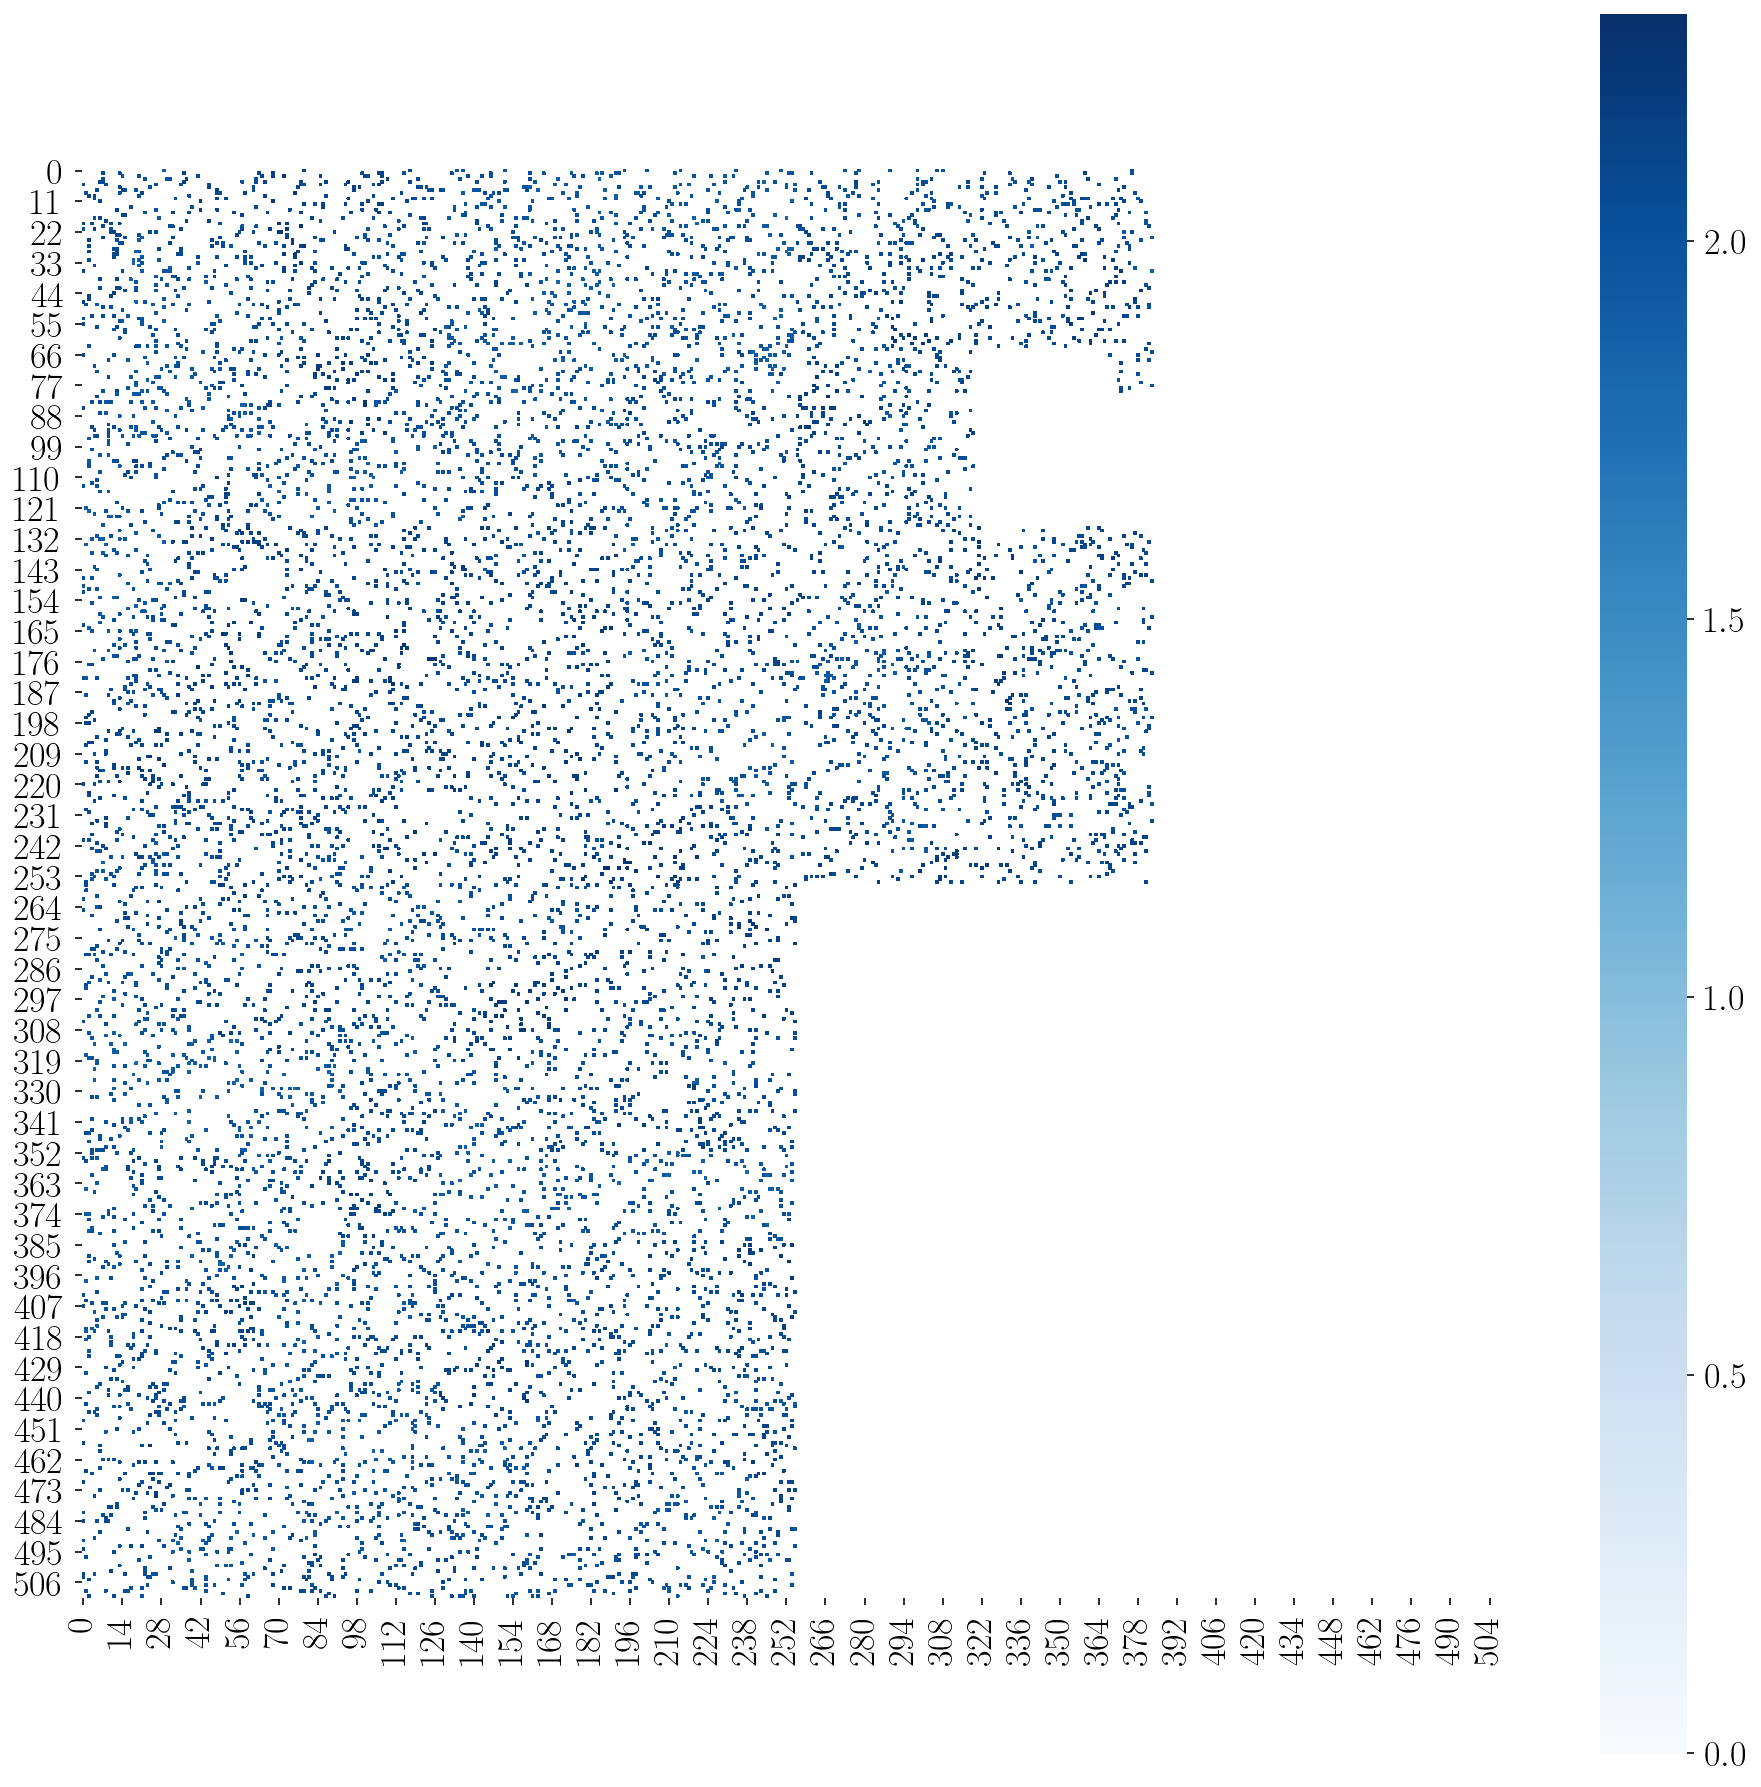
\includegraphics[width=\linewidth]{figures/random_hilbert.png}
    \caption{}
  \end{subfigure}
  \hfill
  % Fig b.
  \begin{subfigure}[b]{.49\linewidth}
    \centering
    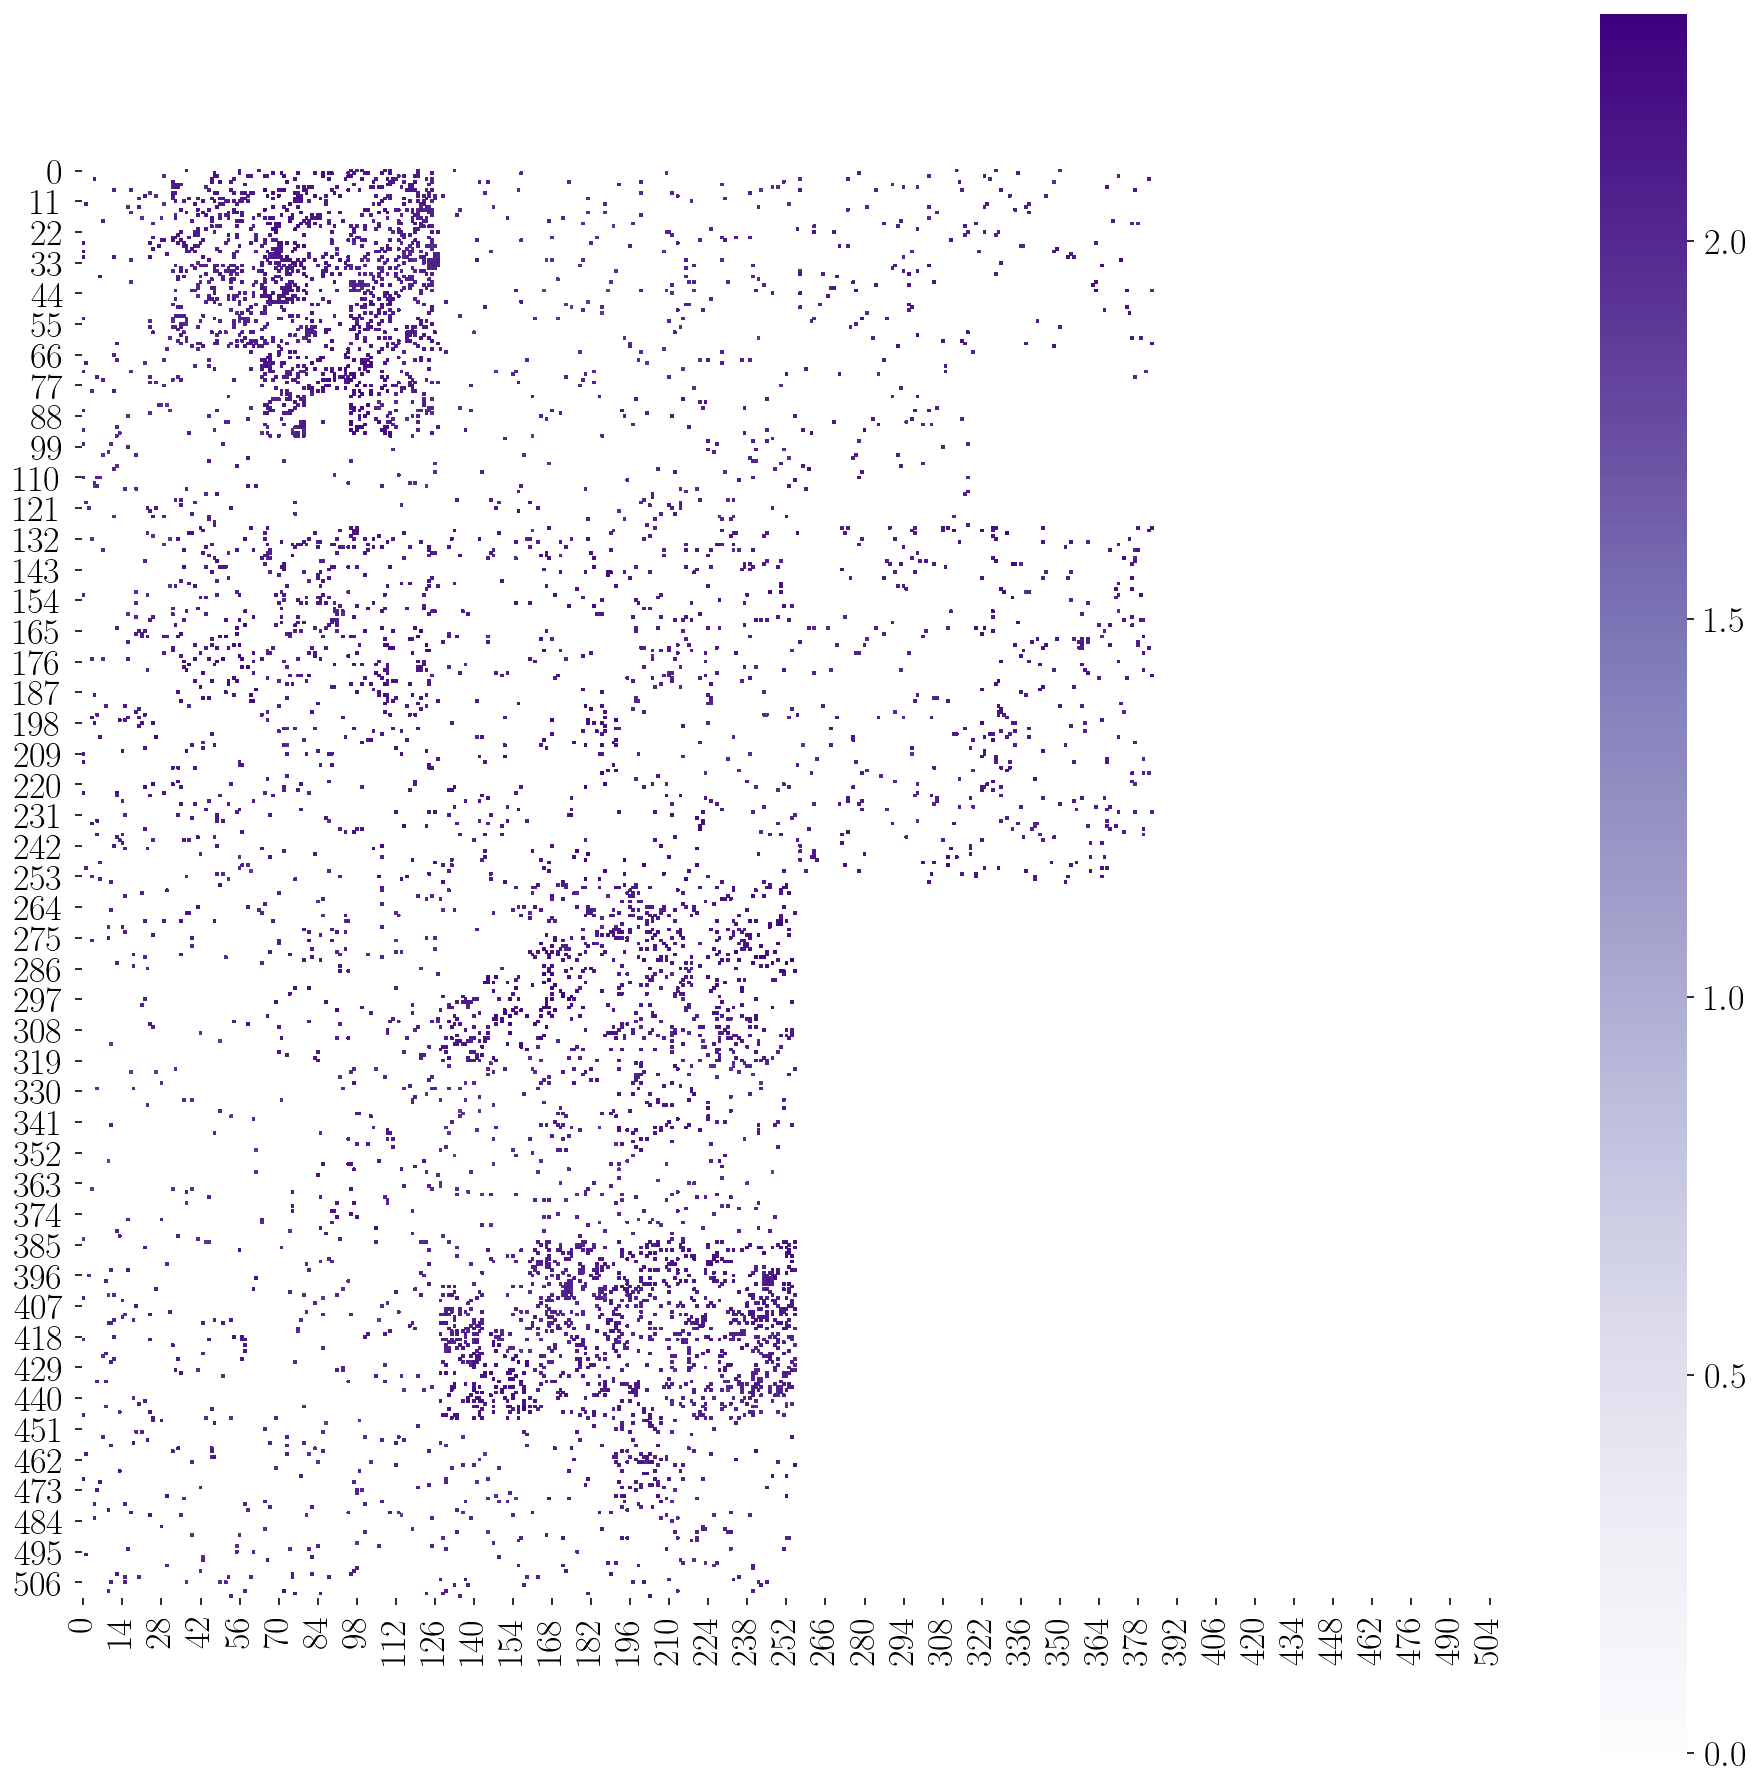
\includegraphics[width=\linewidth]{figures/cbas_hilbert.png}
    \caption{}
  \end{subfigure}
  % Caption
  \caption{
    \textbf{Optimized search.} Protein sequences sampled uniformly \textbf{(a)}
    and using the CbAS optimization scheme \textbf{(b)} from the search space
    projected onto a order 9 Hilbert curve. Compared
    to the random search, the CbAS method quickly localizes its search space to
    regions where it thinks may contain feasible variants, leading to more
    efficient querying. This is especially beneficial for expensive-to-run
    querying tasks. Darker colors indicate higher (oracle) fitness scores.
  }
  \label{fig:landscape_hilbert}
\end{figure}

Beyond the top $k$ sequences, when comparing the variants explored by the CbAS
sample strategy versus the random strategy, we notice in
\cref{fig:random_vs_designed} that the designed variants are likely to be
``better'' (in terms of fitness score) than the wildtype (WT) sequence. In fact,
for variants with a relativey high amount of mutations, the adaptive sampling
scheme seemingly outperforms the random search. This, along with the results
above, suggests that the CbAS algorithm was (a) not led into untrusthworthy
regions of the search space, and, more importantly, (b) more effectively able to
design sequences for a specified design criteria.

\begin{figure}[htbp]
  \centering
  % Fig a
  \begin{subfigure}[b]{.41\linewidth}
    \centering
    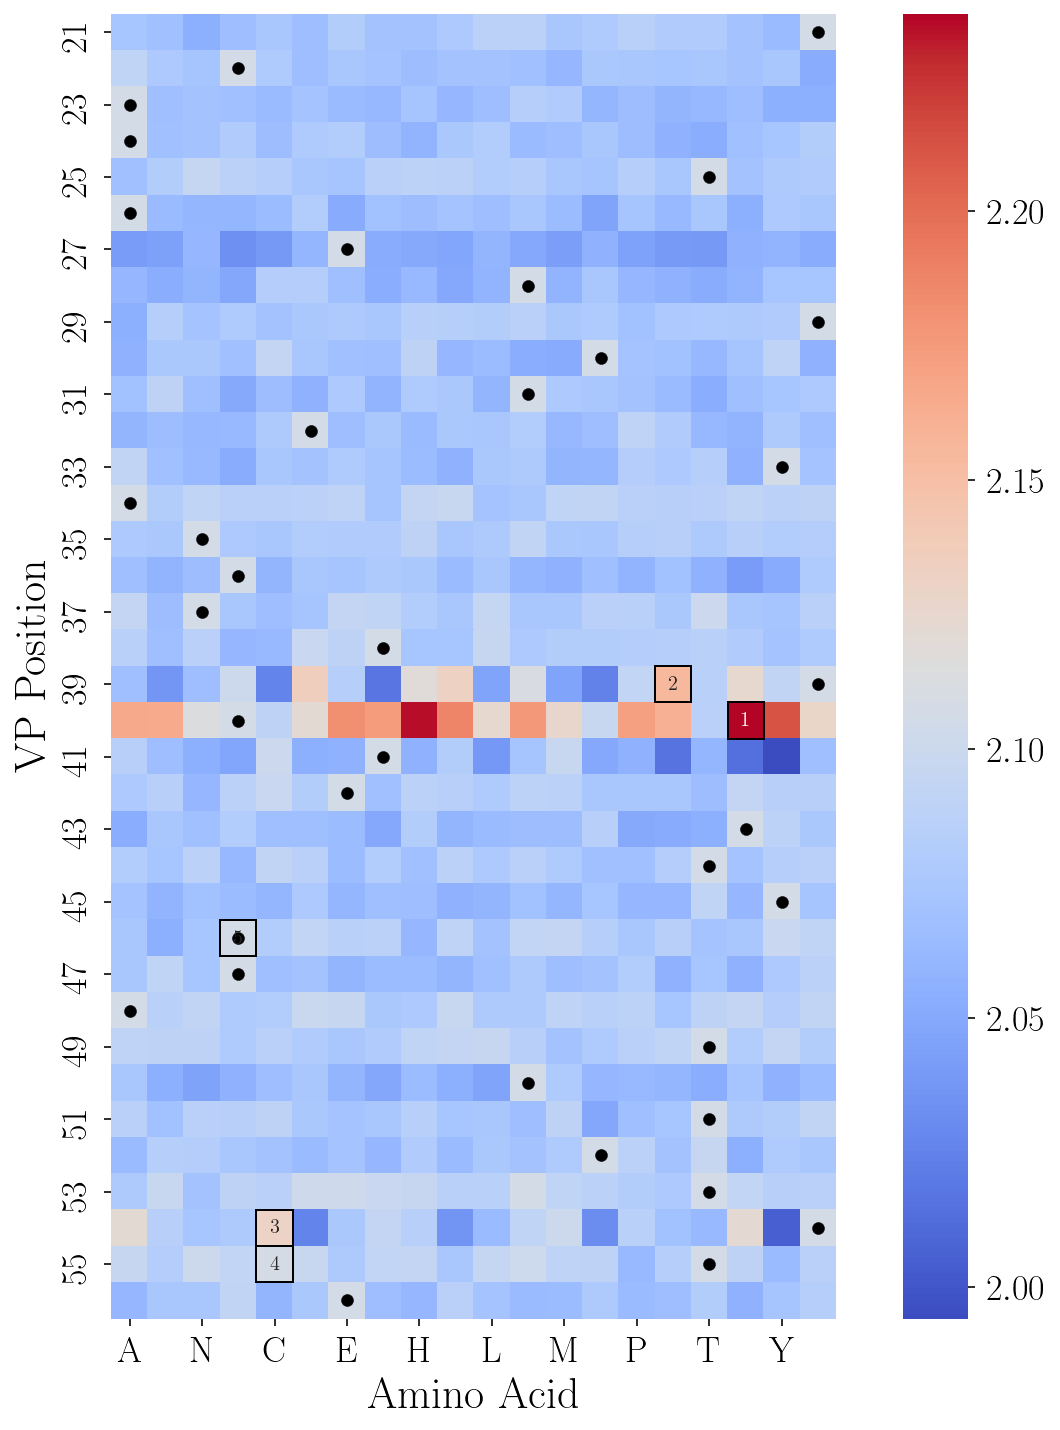
\includegraphics[width=\linewidth]{figures/random_vs_designed_heatmap.png}
    \caption{}
  \end{subfigure}
  \hfill
  % Fig b
  \begin{subfigure}[b]{.57\linewidth}
    \centering
    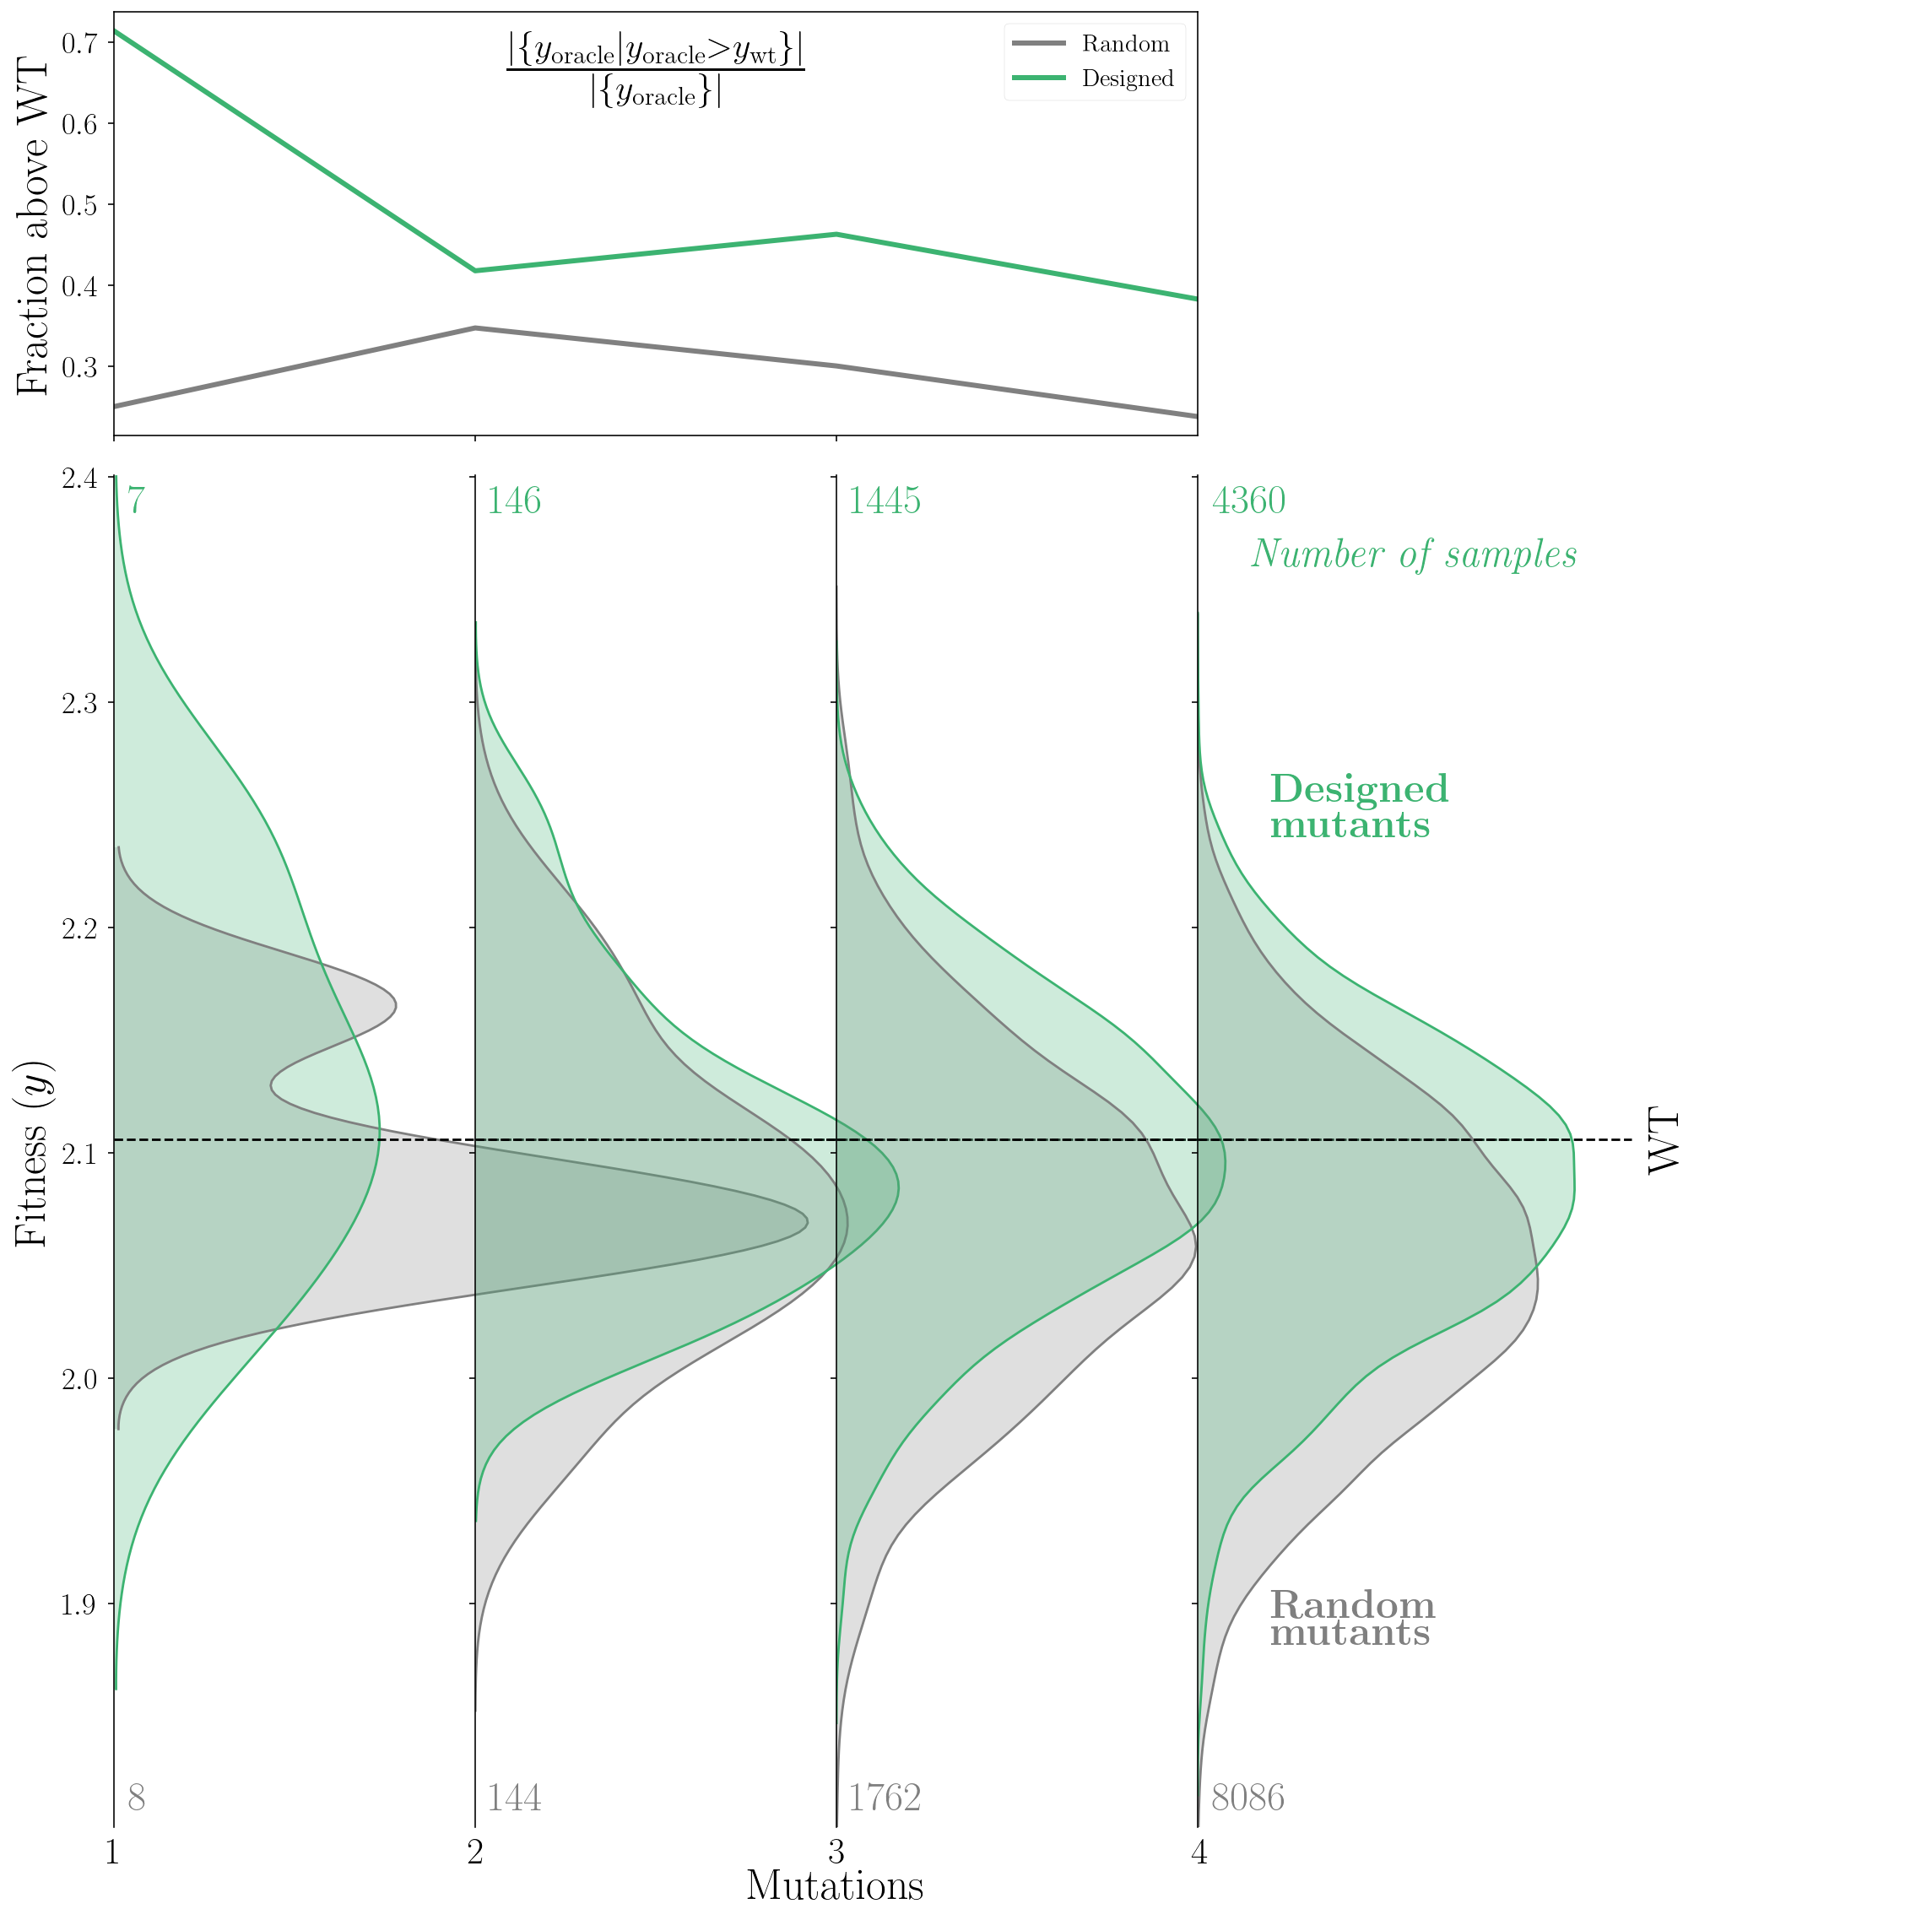
\includegraphics[width=\linewidth]{figures/random_vs_designed_oracle.png}
    \caption{}
  \end{subfigure}
  % Caption
  \caption{
    \textbf{Machine-guided design outperforms random mutagenesis. (a)}
    Multimutant sequence generation from individual amino-acid substitutions
    (black dots: WT). Fitness scores for each position are computed from the
    single amino-acid mutants. Sampled mutations are combined to generate a
    multimutant variant, which is evaluated on the oracle to determine the
    predicted fitness. The top 5 mutations (at different positions) are
    highlighted to show one possible variant. \textbf{(b)} Top: Fraction of
    designed mutants with fitness values greater than WT for random (grey) and
    machine-guided design mutants (green). Bottom: Distribution of fitness
    values for random and designed mutants separated by number of mutations.
    Even at the higher-end of mutation distances ($n=4$), there is a seperation
    between the fraction of proteins above WT from designed and random mutants.
  }
  \label{fig:random_vs_designed}
\end{figure}


\section{Discussion}
In this study, we used a gradient-free optimization strategy\footnote{We do use
gradients to train both the oracle and generative models for performance
reasons, but the optimization function itself does not require gradients. As
such, it can easily be used with non-gradient based predicitve models.} to more
efficiently explore a protein's fitness landscape. The statistical framework
gives a grounding to approximate the conditional density even in the presense of
rare events by leveraging the latent variable models structure to compute
importance sampling for models whose densities cannot be computed exactly. Our
experiments reveal that this approach works well under noisy ``oracle''
evaluations, querying regions of discrete search space with high GT scores,
meaning that we can effectively design ``better'' proteins than other commonly
used techniques, i.e. directed evolution. A big benefit with using a
non-differentiable approach is that is allows us to optimize the design space
with a black-box ``oracle'' -- one that provides a simple input to output
mapping, i.e. a wet-lab assay -- meaning that this optimization scheme can be
readily employed as part of a bigger protein design pipeline.

Additionally, due to how the generative model's parameters are updated at each
step, this method can also be employed in a completely unsupervised setting,
where no training set is provided to build the (initial) generative model.
Instead, the prior would be a uniform distribution over the whole search space.
We did not, however, test this setting since it requires that the oracle
predicts the property being measured well, which we cannot guarantee. As such,
it might lead to less-than-optimal results when compared to other
(semi-)supervised methods that use a training dataset.

While this approach does show some promising results navigating the search
space, it does have its drawbacks. In particular, knowing if the algorithm has
converged to the optimal sample (based off its design criteria) is hard to
determine, since we do not know the underlying distribution. This is hightened
by the fact that the search regions the algorithm chooses to explore are
sensitive to (a) the number of iterations and (b) the number of points sampled
per iteration, which directly affects the EvE tradeoff. Additionally, since the
``oracle'' poorly fits the training dataset (see
$\S$\ref{sec:appendix-model_accuracy}), the search model might not perform
optimally since it weights are partially optimized using the oracle's
predictions\footnote{This does not mean that the algorithm is being lead astray
into regions of space which are ``poor'', but rather that the reported fitness
score on the newly sampled variants might not be accurate.}. Unsurprisingly,
this does not affect the regions of the search space the algorithm explores, as
it was designed to avoid pathological behavior of the oracle (see
$\S$\ref{sec:appendix-search_model_opt}).

Although not directly related to the search strategy itself, another big
downside is that we only consider variants with exactly $k$ mutations at the
same amino acid positions. As the algorithm's main objective in
(\ref{eq:latent_approx_opt}) is to minimize the difference between the
generative model's search and the conditional distribution, the samples the
search model generates are not representative of the vast sequence space
($\Theta(20^L)$), but rather only a small subset of proteins ($\Theta(20^4)$).
As such, there is a high likelihood that we miss finding optimal variants which
satisfy our desired property (i.e. maximization of the fitness). In other words,
it can be seen as finding the optimia locally rather than globally (since we do
not have data sampled from the full search space to build our initial prior
model).

We are working on further extensions of the approach, by using techniques found
in the reinforcement learning literature \cite{koulouriotis2008reinforcement,
kuleshov2014algorithms}. In particular, to tackle the EvE-tradeoff, we plan on
using upper confidence bounds (UCB) \cite{auer2010ucb} to prefer actions for
which we don't have confident value estimates for, favoring exploration of
samples with a strong potential to have great values. In a more nuanced flavor,
since we have knowledge of the prior distribution, we can make better estimates
of the bounds, allowing us to set the upper bound as the $95\%$ confidence
interval \cite{kaufmann2012bayesian}. Finally, using the Thompson sampling
scheme could also allow us to select events $e$ based off its optimality
probability, choosing samples that maximize the expected reward with respect to
a randomly drawn belief \cite{agrawal2012analysis}.

While reinforcement learning techniques allow for better exploration strategies,
simpler modifications, such as using domain-specific biochemistry knowledge, can
make the oracle more accurate. For example, a model that incorporates the 3D
structural features of the protein \cite{cho2018three} could be used, owing to
the fact that structure affects function, which, in turn, affects the overall
protein's fitness. More specifically, consider the chemical differences between
different amino acids. When substituting certain amino acids with others, where
a non-polar R-group is substituted with another non-polar R-group, the overall
structure of the protein might not change by much \cite{betts2003amino,
loladze2002thermodynamic}. On the other hand, with a polar R-group modification,
the structure might change just enough to affect the overall fitness
\cite{alvares2013effects}. Overall, any model that is best able to learn an
encoded representation of the protein (i.e. Unirep \cite{alley2019unified})
would be useful for a lot of downstream tasks.


\section{Acknowledgements}
We thank Brookes et. al. for useful clarifications and for providing python
scripts\footnote{\url{https://github.com/dhbrookes/CbAS}} that served as a base
to reproduce the CbAS method presented in \cite{brookes2019conditioning}. It is
important to stress that all we have done is adapted their method to work on the
dataset complied in \cite{wu2016adaptation}. We also like to thank the authors
of \cite{ogden2019comprehensive} for the inspiring the design of
\cref{fig:random_vs_designed}.

% References
\bibliographystyle{unsrt}
\bibliography{./references.bib}


% Appendix
\newpage
\appendix

\section{Appendix}

\subsection{Model accuracy}
\label{sec:appendix-model_accuracy}
The oracle is a densely-connected neural network trained on one-hot encoded
representations of the protein sequence. It is evident from
\cref{fig:model_selection} that the oracle was poorly trained, despite the fact
that the model's validation loss was relatively low for each run. In fact, even
after correcting for imbalanced samples (since most samples have a low fitness
score), the oracle's predictions were still subpar when compared to the true
fitness value, increasing by approximately the same amount for every sample. As
such, there is very little variance in the fitness score prediction between
samples.

This is remarkably different from the GPR, which shows great correspondence with
the training dataset. In fact, for most subsets of the dataset with which it was
trained on, the GPR is well-behaved (atleast within the domain shown). This
suggests that, the oracle did not capture what makes a sequence ``good'' vs
``bad'' in terms of its fitness, while the GPR was better able to make the
distinction. Overall, this suggests, for optimality, we should choose the
oracle's parameters trained on values greater than the mean, and the GPR's
parameters on values greater than zero.

\begin{figure}[htbp]
  \centering
  % Fig a
  \begin{subfigure}[b]{\linewidth}
    \centering
    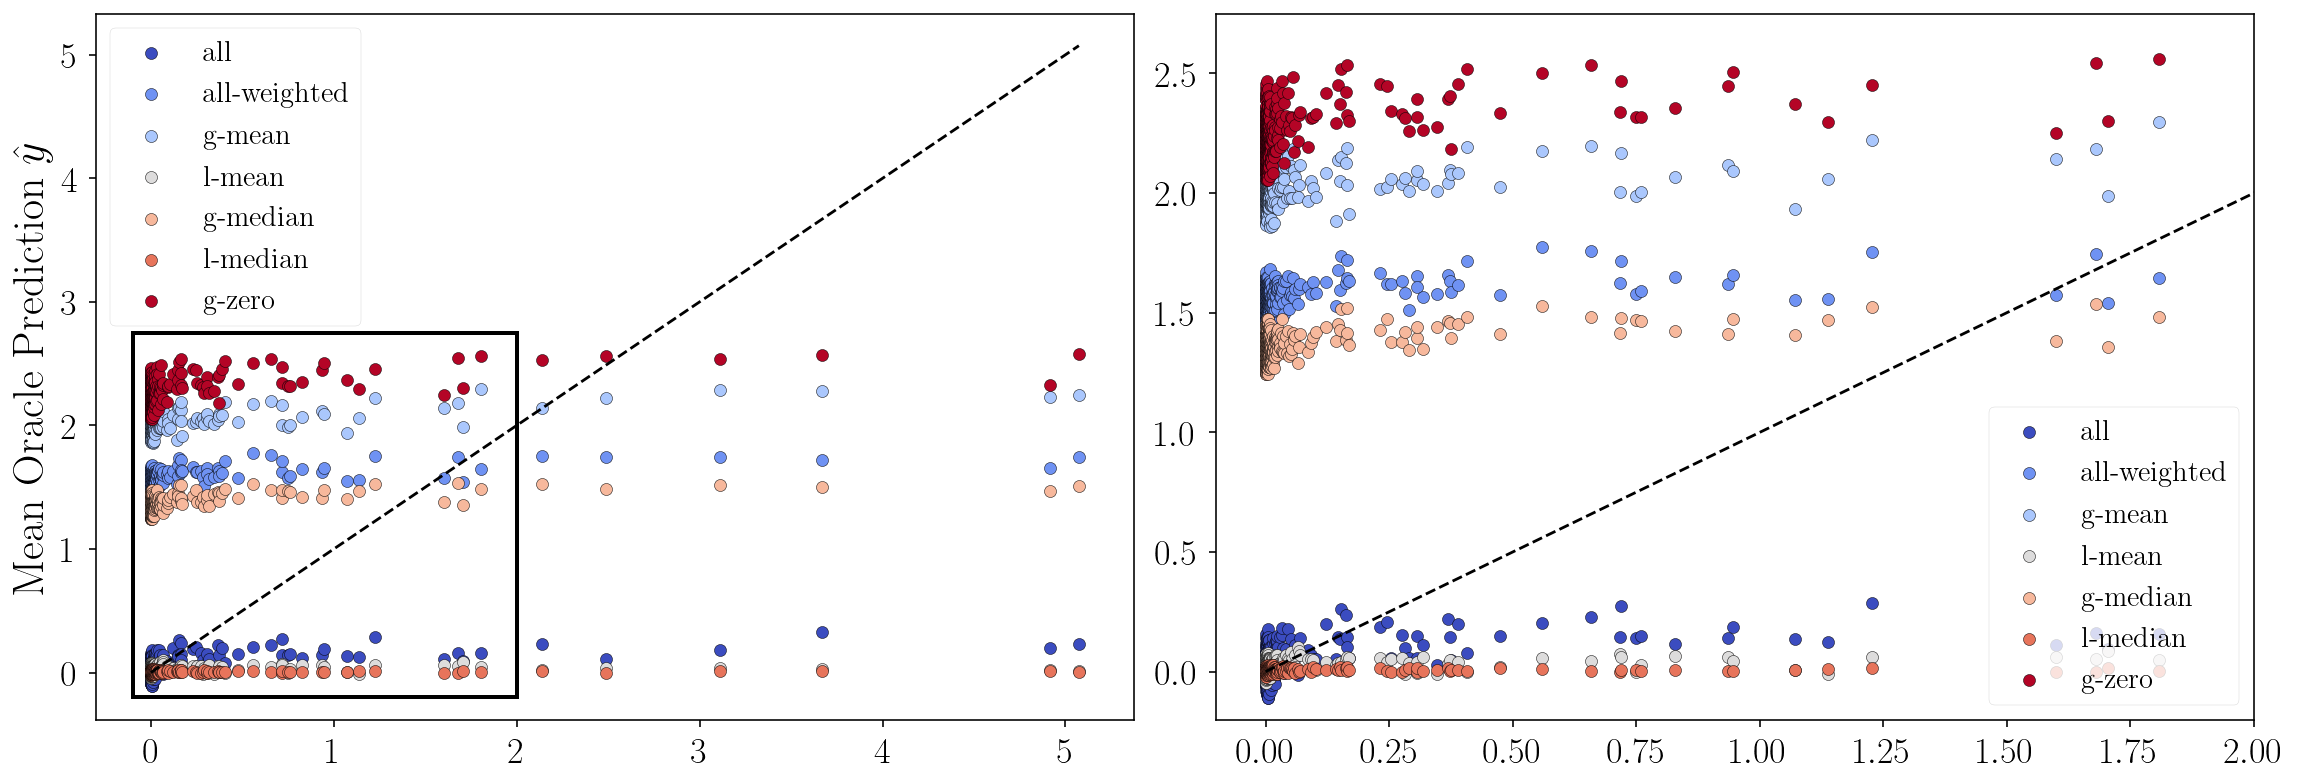
\includegraphics[width=\linewidth]{figures/oracle_pred_vs_gt.png}
    \caption{}
  \end{subfigure}
  \vspace{2mm}
  % Fig b
  \begin{subfigure}[b]{\linewidth}
    \centering
    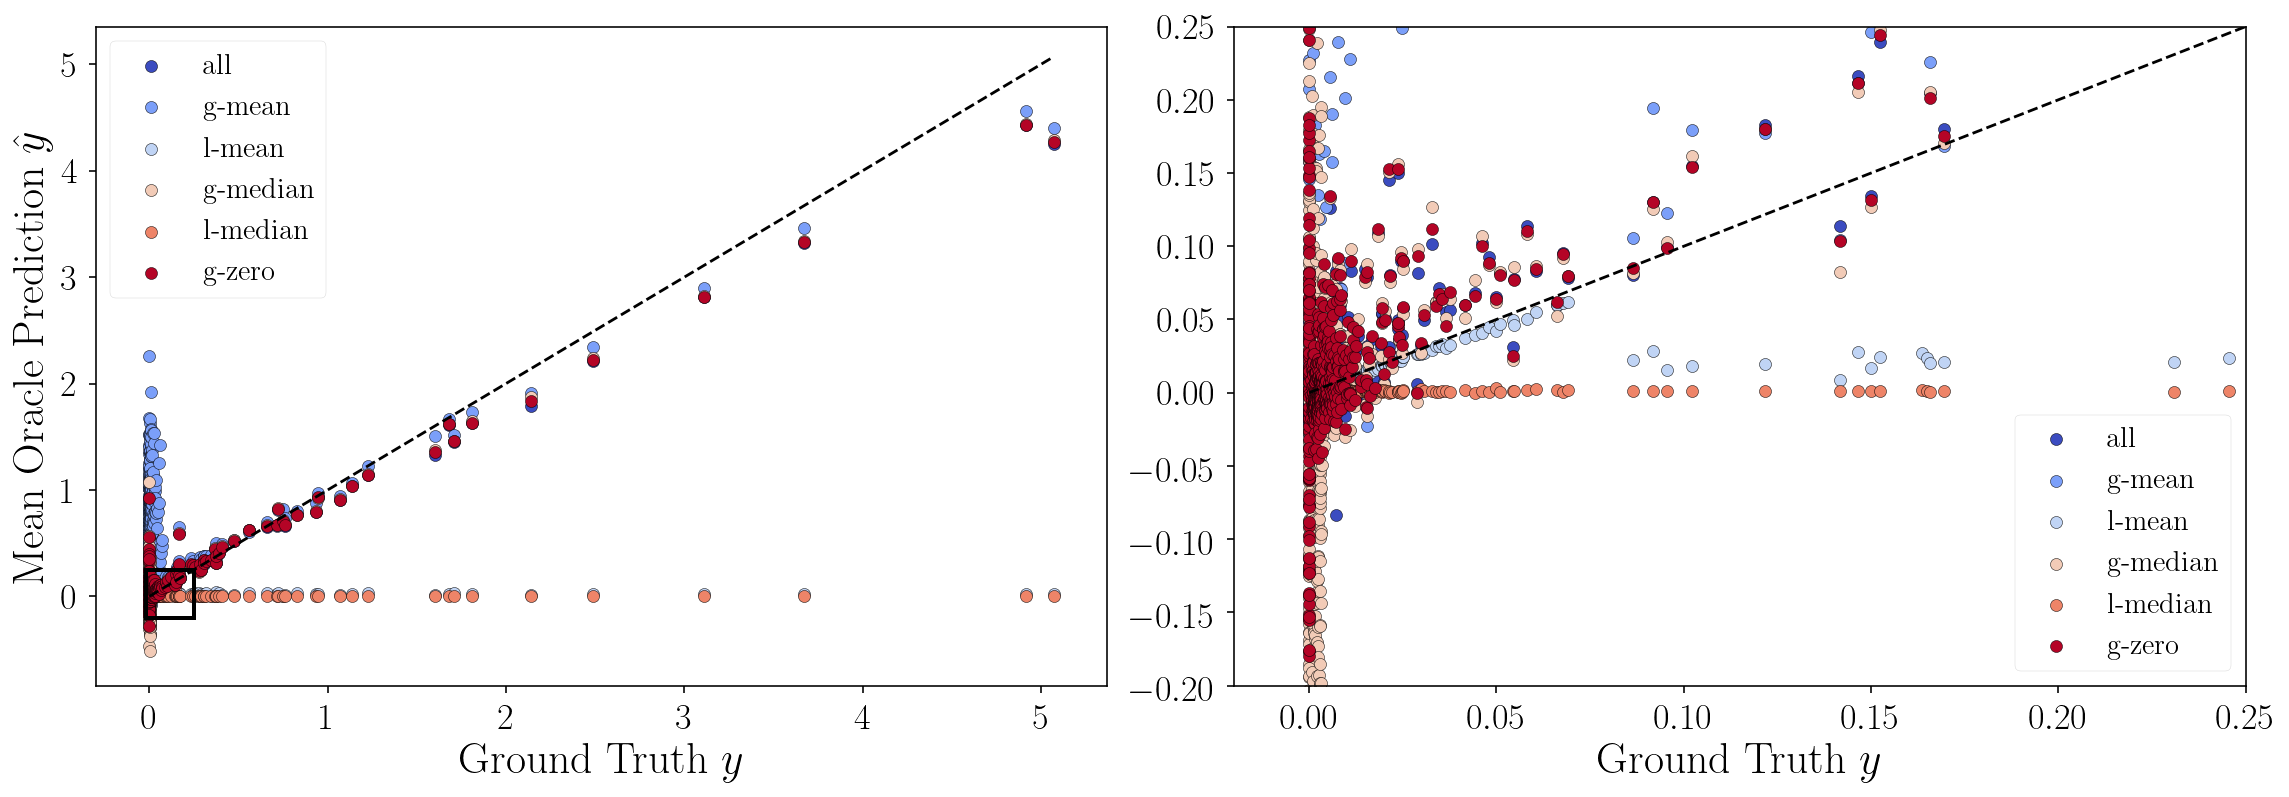
\includegraphics[width=\linewidth]{figures/gpr_pred_vs_gt.png}
    \caption{}
  \end{subfigure}
  % Caption
  \caption{\textbf{Model selection.} Predicted vs. ground truth fitness score
    for samples trained on different subsets of the training data. In (a),
    irrespective of the GT fitness score, most predictions are the same, while
    the GPR model in (b) shows better alignment between the predicted and ground
    truth values. The dashed line denotes what an ideal model will predict (aka
    $\hat{y} = y$ for both the predicted and true values). The figures on the
    right show the zoomed in view of the bounding boxes shown on the left.}
  \label{fig:model_selection}
\end{figure}

\subsection{Search model optimization}
\label{sec:appendix-search_model_opt}
To measure how well the search model is optimized, we measure both the oracle
and GP predictions (a proxy for the GT) for each sequence sampled at every
iteration $t$. \cref{fig:search_model_qth_percentile} shows the $80^{\text{th}}$
percentile for both the oracle and GT values across different runs of the
algorithm, which use different models trained on various subsets of the training
data. As intended per the formulation, the results indicate that the search
strategy does not get led into pathological regions of the search space since
the GT values remain consistently high even after a certain score is reached.
If, instead, the GT values were to decrease substantially, this would indicate
that the algorithm is being negatively influenced by the oracle's inconsistent
behavior.

\begin{figure}[htbp]
  \centering
  % Fig a
  \begin{subfigure}[b]{0.49\linewidth}
    \centering
    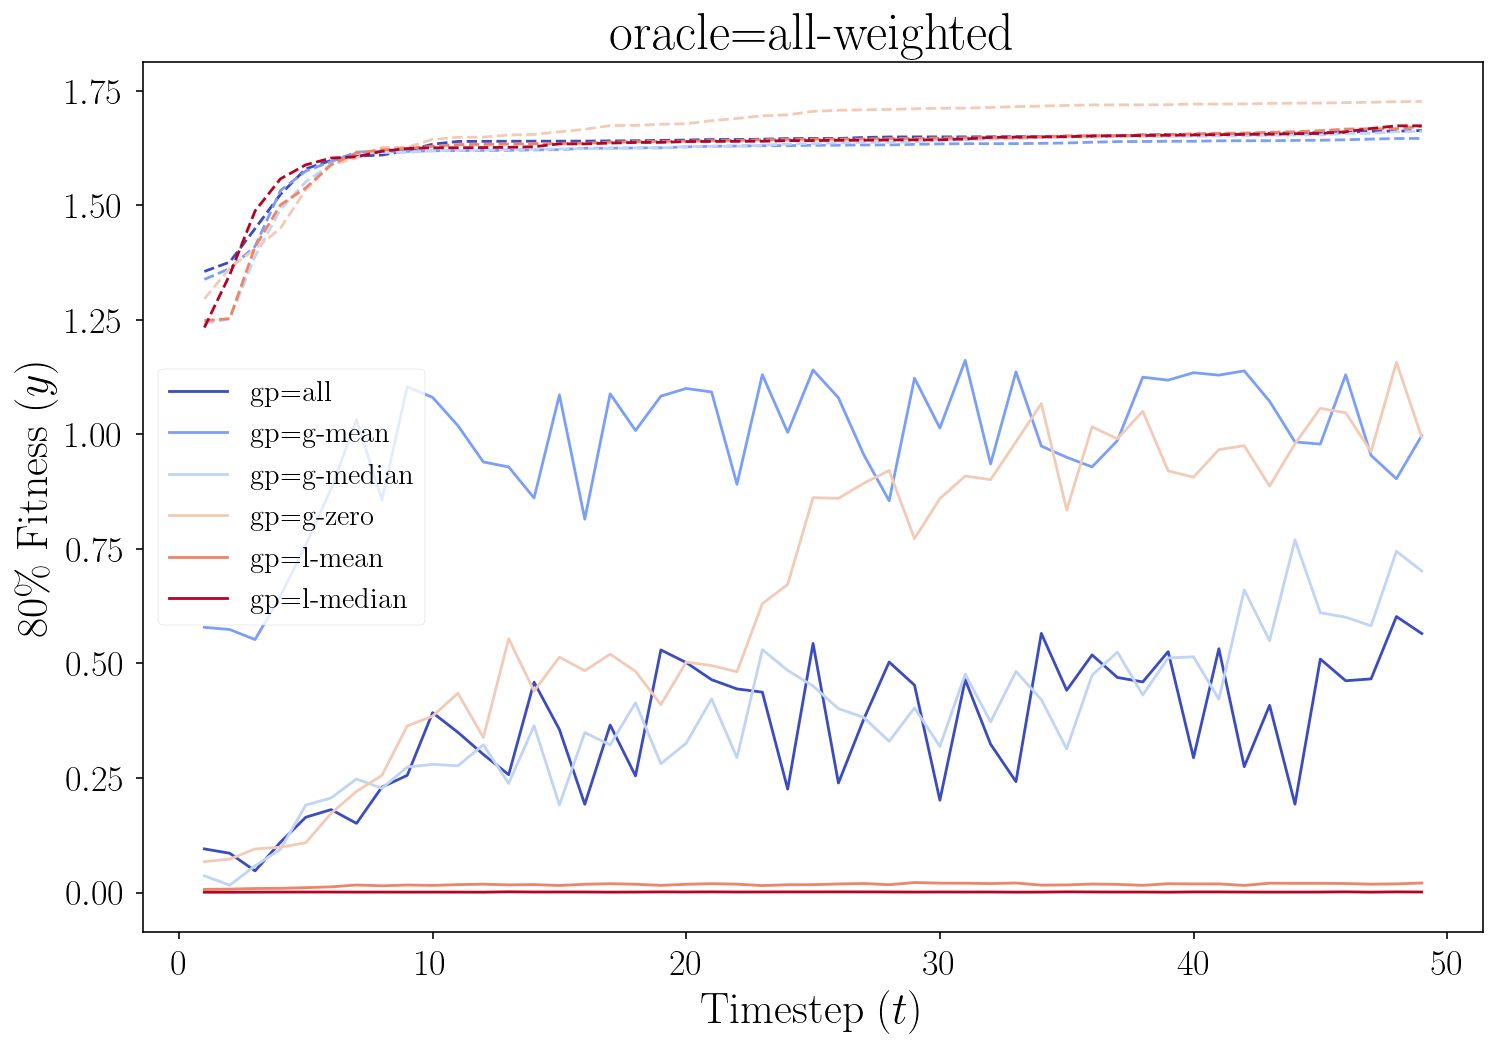
\includegraphics[width=\linewidth]{figures/pred_vs_gt_fitness_explored(all).png}
  \end{subfigure}
  \hfill
  % Fig b
  \begin{subfigure}[b]{0.49\linewidth}
    \centering
    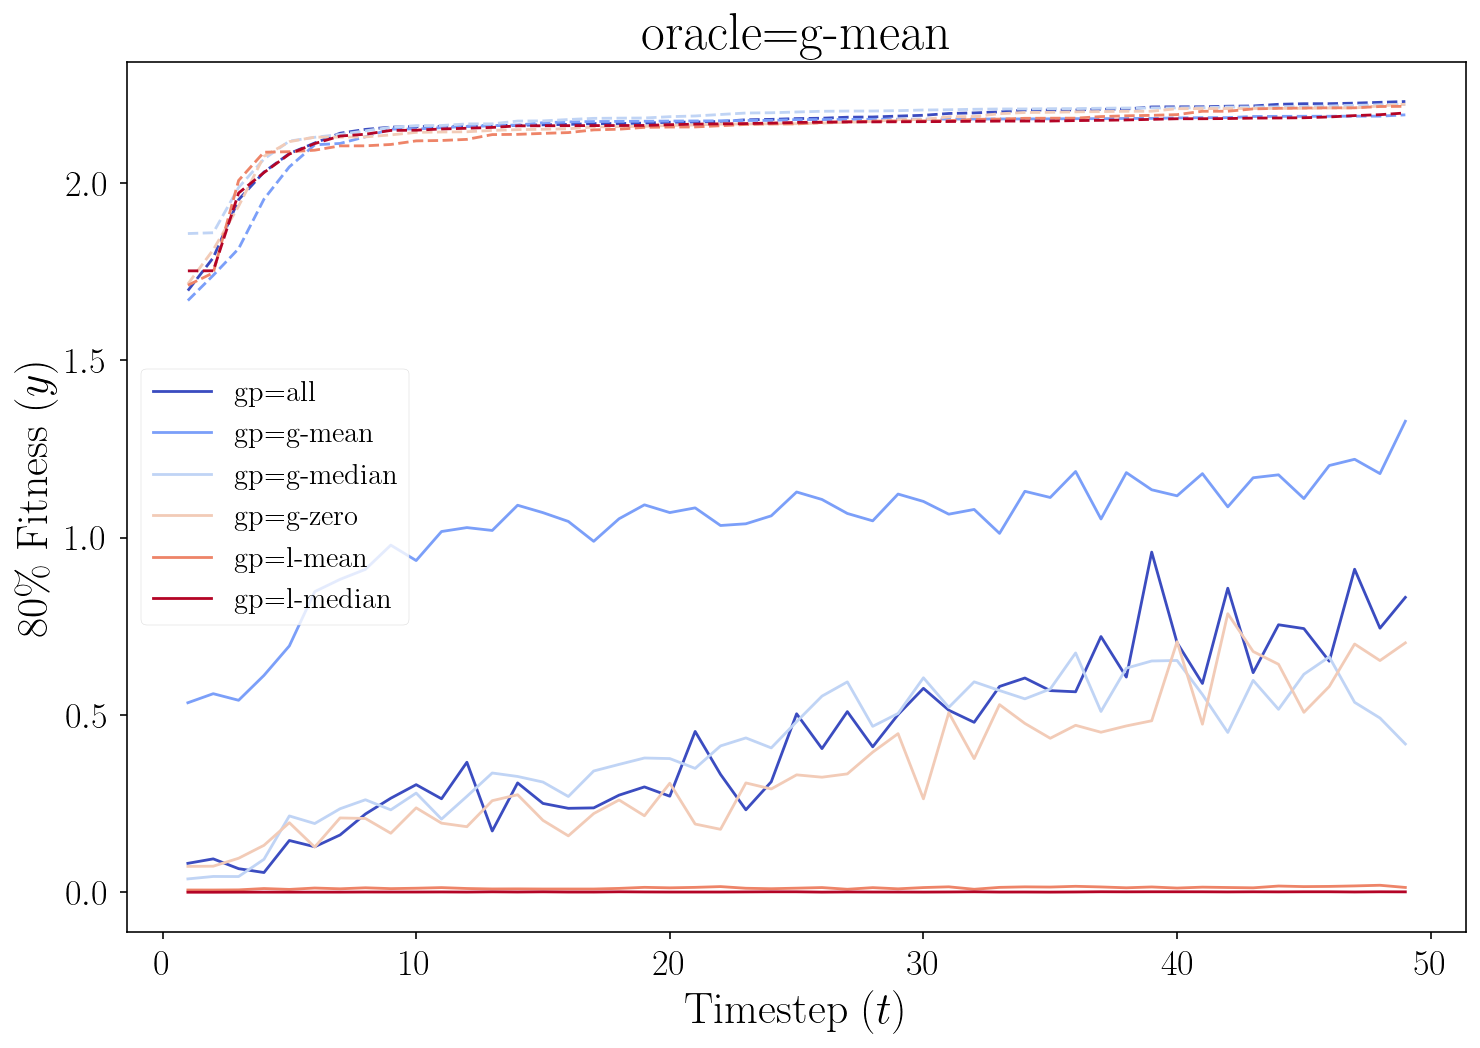
\includegraphics[width=\linewidth]{figures/pred_vs_gt_fitness_explored(mean).png}
  \end{subfigure}
  \vspace{2mm}
  % Fig c
  \begin{subfigure}[b]{0.49\linewidth}
    \centering
    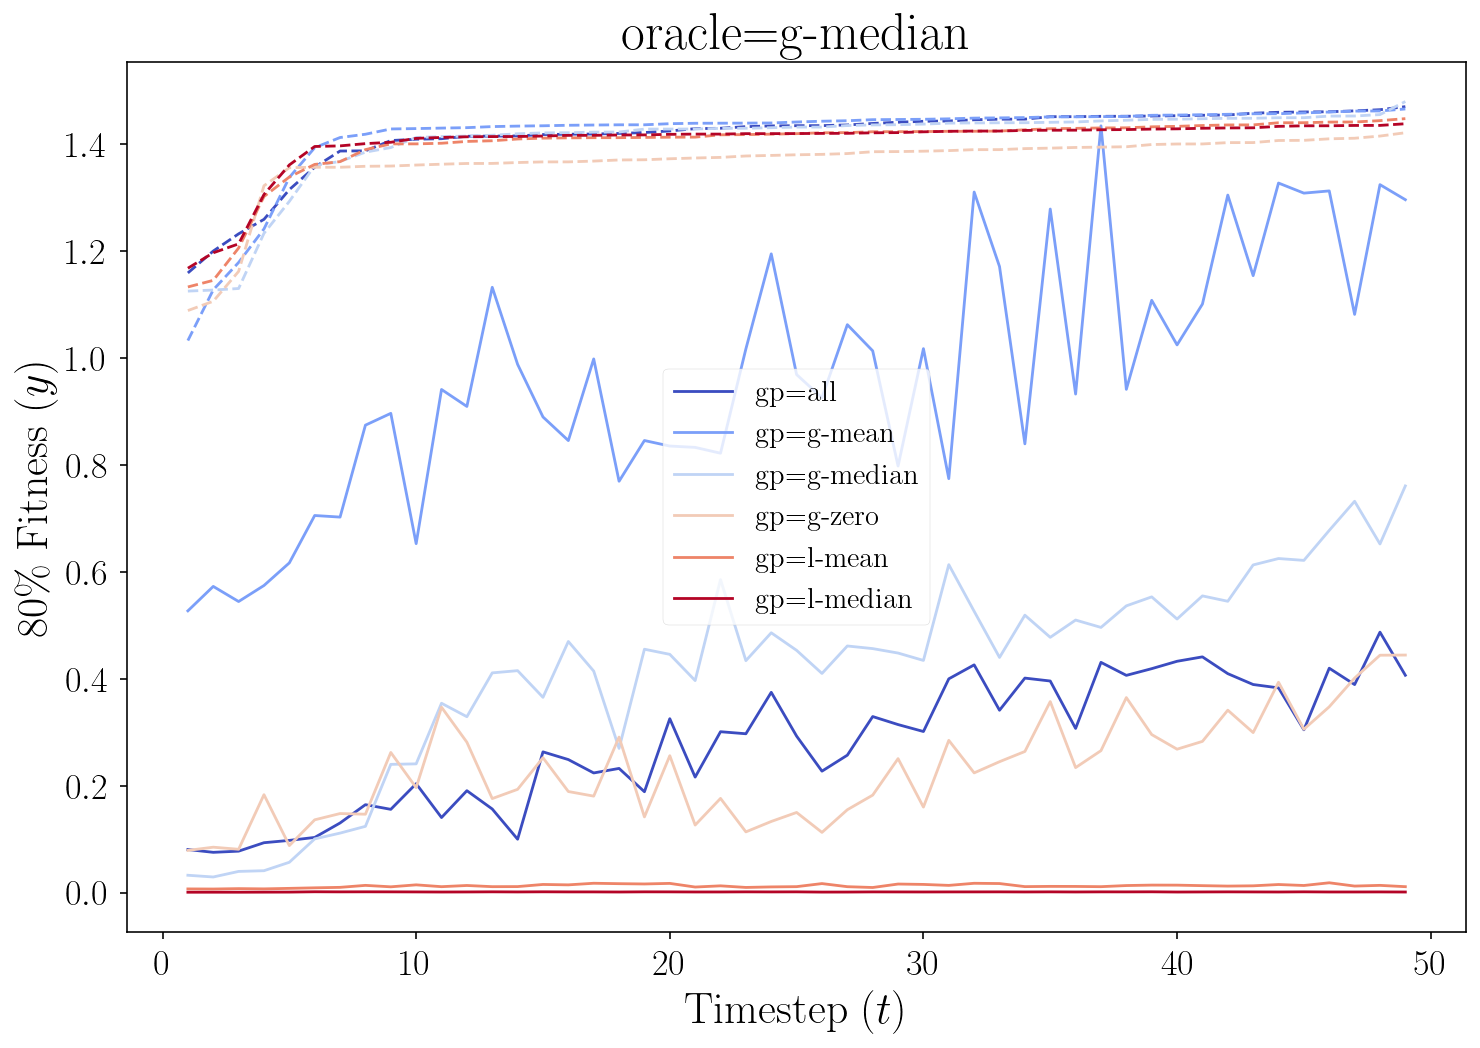
\includegraphics[width=\linewidth]{figures/pred_vs_gt_fitness_explored(median).png}
  \end{subfigure}
  \hfill
  \begin{subfigure}[b]{0.49\linewidth}
    \centering
    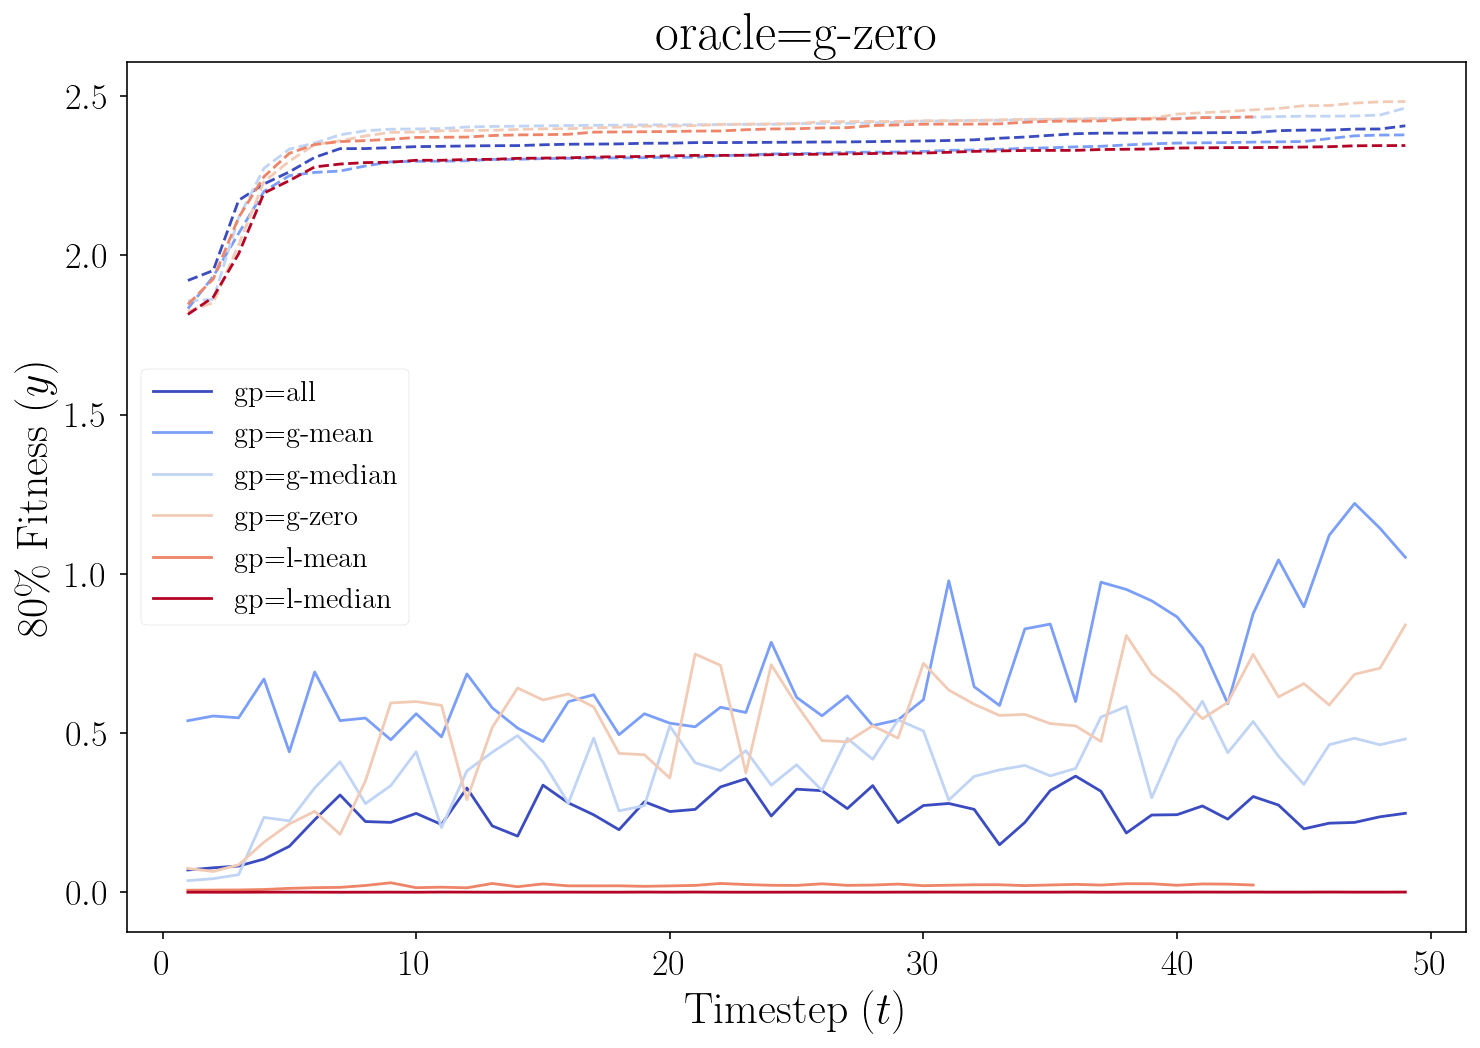
\includegraphics[width=\linewidth]{figures/pred_vs_gt_fitness_explored(zero).png}
  \end{subfigure}
  \caption{
    \textbf{Maximization of protein fitness.} Trajectory plots of runs for each
    oracle. Each line (within a panel) represents the algorithm's trajectory for
    a specific run of the GP trained on a subset of the original data. Each
    point in the dashed line represents the $80^{\text{th}}$ percentile of
    oracle evaluations at that iteration. The cooresponding point on the solid
    line indicates the mean ground truth value as computed by the GPR. The
    trajectory is sorted by increasing oracle values such that the last point on
    the curve represents the final designed variant that would be used (in this
    case the highest oracle value predicted). This is done because the ground
    truth values would be unknown in a real-world setting.
  }
  \label{fig:search_model_qth_percentile}
\end{figure}

\subsection{Variants that could improve the model}
\label{sec:appendix-variants}
Taking into account the algorithm's limitations, the most immediate improvement
can likely be made by using a more representative training dataset (i.e. one
that contains variants that have a high fitness score) to help balance the
dataset. Not only would this improve the prior generative model's parameters
(generating better initial samples), but also the accuracy of the oracle's
predictions, further improving the search model in subsequent iteration cycles.
Ideally, this will help find optimal sample(s) based off the design criteria
more effectively. Alternatively, we could choose to include variants based on
how uncertain we are about a given sample (this is the UCB strategy used in
multi-armed bandit problems). Although not immediately useful to build a more
accurate oracle, it helps sample points quickly to reduce the uncertainty of the
unknowns before ``locking'' onto variants satisfying the property of interest.

\end{document}
